\documentclass[a4paper]{article}

\usepackage{graphicx} 
\usepackage[english]{babel}
\usepackage{graphicx}
\usepackage{float}
\usepackage{amssymb}
\usepackage[a4paper,top=3cm,bottom=2cm,left=2cm,right=2cm,marginparwidth=1.75cm]{geometry}

\begin{document}

\begin{titlepage}
    \newcommand{\HRule}{\rule{\linewidth}{0.5mm}}
    \center

    \textsc{\LARGE Delft University of Technology}\\[1cm]

    \textsc{\Large Reasoning \& Logic}\\[0.2cm]
    \textsc{\large CSE1300}\\[1cm]
    \HRule \\[0.8cm]
    { \huge \bfseries Assignment: TA-check 2}\\[0.7cm]
    \HRule \\[2cm]
    \large
    \emph{Authors:}\\
    Joris Rijs (5880998) \& Sebastiaan Beekman (5885116)\\[1.5cm]
    {\large \today}\\[5cm]
    
\includegraphics[width=0.6\textwidth]{images/TU_delft_logo.jpg}\\[1cm]
    \vfill
\end{titlepage}

\newpage
\tableofcontents

\newpage
\section{Question 1}

\newpage
\section{Question 2 - Tarski's World}
\subsection{(a)}
In Tarski's world, it is possible to describe situations using formulas whose truth can be evaluated,
which are expressed in a first-order language that uses predicates such as Rightof(x,y),
which means that x is situated—somewhere, not necessarily directly—to the right of y, or Blue(x), which means that x is blue.
In the world in Figure 2.9 in Delftse Foundations of Computation (p. 30), for instance,
the formula$\forall $x(Triangle(x) $\rightarrow $ Blue(x)) holds, since all triangles are blue, but the converse of this
formula, $\forall $x(Blue(x) $\rightarrow $ Triangle(x)), does not hold, since object c is blue but not a triangle.

\begin{figure}[H]
    \centering
    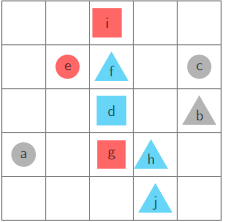
\includegraphics[]{images/tarski-world-example-1.png}
    \caption{An instance of a Tarski World.}
    \label{fig:Tarski}
\end{figure}
\ \\
\textbf{Alfred Tarski} contributed much to the semantics of first-order languages and the systematic development of the concept of truth.
In the program Tarski's World, described in the book Language, Proof and Logic by Barwise and Etchemendy,
a 'Tarski World' is a visualization of a 'mathematical structure,' a core concept in that theory: a structure is a description of a 'situation' wherein one can
evaluate whether a statement in a given first-order language (say, T) is true or false. A structure
contains a domain with objects, plus an indication of all (combinations of) objects with the properties
denoted by the predicate symbols in the language T: Blue(a) is true in a structure (e.g. named A) in
which the object with the name 'a' belongs to the set of objects with the property of being blue. That
set is called $B^A$: the set in structure A that indicates which objects have the property indicated by
predicate symbol B. In Tarski's World, color indicates to which set each object belongs, which could
be notated more generally by describing the set B as $B^A$ = \{a,c,e,g\}. The relation that corresponds
to the predicate RightOf is indicated by the positioning between the objects, but this can be denoted
more generally by describing the relation as the set (see chapter 1) of all pairs (x,y) $\in $ D x D for
which x is situated right of y in the picture: $RightOf^A$ = \{(b,a), (c,a), (d,a), (c,f),...\}.
\subsubsection{(I)}
Give the structure that is visualized in Figure 1 (of this document) in the abstract way
as described above. Take another good look at section 2.4.4 in the book, where you can find
explanations about what this should entail. You may leave out LeftOf, AboveOf, and BelowOf.
\\\\
D = \{a,b,c,d,e,f,g,h,i,j\}\\
$Blue^A$ = \{d,f,h,j\}\\
$Red^A$ = \{e,g,i\}\\
$Grey^A$ = \{a,b,c\}\\
$Square^A$ = \{d,g,i\}\\
$Circle^A$ = \{a,c,e\}\\
$Triangle^A$ = \{b,f,h,j\}\\
$RightOf^A$ = \{(b,a), (c,a), (d,a), (e,a), (f,a), (g,a), (h,a), (i,a), (j,a), (b,e), (c,e), (d,e), (f,e), (g,e), (h,e), (i,e), (j,e), (b,i), (c,i), (h,i), (j,i), (b,f), (c,f), (h,f), (j,f), (b,d), (c,d), (h,d), (j,d), (b,g), (c,g), (h,g), (j,g), (b,h), (c,h), (b,j), (c,j)\}
\subsubsection{(II)}
D = \{a,b\}\\
$Blue^B$ = \{a\}\\
$Grey^B$ = \{b\}\\
$Square^B$ = \{b\}\\
$Triangle^B$ = \{a\}
\\\\
Arguments:
\begin{itemize}
    \item $\exists $x(Triangle(x) $\vee $ Blue(x)), see a
    \item $\exists $x(Square(x) $\wedge $ Grey(x)), see b
    \item $\forall $y(Circle(y) $\rightarrow $ Red(y)), no circles
    \item $\forall $z(Triangle(x) $\rightarrow $ $\neg $Grey(z)), see a
\end{itemize}
\subsubsection{(III)}
A counter example is a Tarski World with a single entity. An entity can never be left or right of itself, so in the claim $\forall $x$\forall $y(RightOf(x,y) $\leftrightarrow $ LeftOf(x,y)) one side is always false and the other is always true (due to the not). This means that the claim is false.

\newpage
\subsection{(b)}
For the following invalid arguments, give suitable counterexamples. A counterexample is a structure
as in question 'a', in which all premises (if any) hold, while the conclusion does not hold. You also
need to specify which sets in your structure correspond to which predicate symbols in the formulas.
Note that the domain of a structure cannot be empty. Each time, explain why your structure forms
a counterexample.
\\\\
As an example consider the following argument:\\
$\exists $x(P(x) $\wedge $ Q(x)), $\forall $x(Q(x) $\rightarrow $ R(x)) $\therefore $ $\forall $x(P(x) $\rightarrow $ R(x))
\\\\
What's being claimed is that if there is an object with property P that it also has property Q, and
all objects that have Q also have R, then all all objects with P have R as well. This is clearly not
the case, as is shown by the following structure C with domain D = \{4, 5\}. Let $P^c$ = \{4, 5\} and
$Q^c$ = $R^c$ = \{4\}. Now the first premise holds (take x = 4), the second one holds as $Q^c$ = $R^c$, but
the conclusion does not hold: take x = 5.\\
\subsubsection{(I). }

\subsubsection{(II). }

\subsubsection{(III). }

\subsubsection{(IV). }

\subsubsection{(V). }

\newpage
\section{Question 3}

\newpage
\section{Question 4}

\newpage
\section{Question 5}

\end{document}